La pianificazione è stata stilata in base alle scadenze preventivate al punto 1.4 del documento. Si è deciso di dividere il processo di sviluppo in cinque fasi:
\begin{itemize}
    \item \textbf{Analisi};
    \item \textbf{Analisi di dettaglio};
    \item \textbf{Progettazione della base tecnologica};
    \item \textbf{Progettazione di dettaglio e codifica};
    \item \textbf{Validazione e collaudo}.
\end{itemize}
Ogni fase prevede periodi di incremento e successiva validazione delle attività in essa previste. Questi verranno riportati in \citgl{diagrammi di Gantt}, ciascuno dedicato ad una fase specifica. Per ogni fase e rispettive attività verranno indicati i ruoli che contribuiranno all'avanzamento. La scadenza di ogni fase è segnata come \citgl{milestone}.
\subsection{Analisi}
La fase di Analisi ha inizio in data 04-03-2019 e termina il 01-04-2019. I ruoli attivi in questa fase sono:
\begin{itemize}
    \item \textbf{Responsabile di progetto};
    \item \textbf{Amministratore};
    \item \textbf{Verificatore};
    \item\textbf{Analista}.
\end{itemize}
Le attività svolte in questa fase sono:
\begin{itemize}
    \item \textbf{Norme di Progetto}: Consiste nella stesura di un documento da parte degli Amministratori. Questa attività ha la priorità e risulta bloccante all'inizio delle altre attività previste in questa fase, ad eccezione dell'incremento del Glossario. Ciò è dovuto alla natura del documento, che consiste nella stesura di una serie di norme e strumenti che dovranno essere utilizzate dai membri del gruppo in tutte le attività dello sviluppo al fine di garantire qualità e uniformità nella forma dei contenuti;
    \item \textbf{Studio di Fattibilità}: Consiste nella stesura di un documento da parte degli Analisti in cui, per ogni capitolato proposto al gruppo viene effettuato uno studio di fattibilità. Da questo studio risulterà la scelta di un unico progetto che il gruppo si impegnerà a sviluppare;
    \item \textbf{Analisi dei Requisiti}: Consiste nella stesura di un documento da parte degli Analisti. Il contenuto è ricavato dallo studio approfondito dei requisiti richiesti dal progetto facente riferimento al capitolato scelto nello Studio di Fattibilità;
    \item \textbf{Piano di Progetto}: Consiste nella stesura di un documento da parte del Responsabile di Progetto, con l'aiuto degli Amministratori. Consiste nell'analisi delle attività necessarie allo sviluppo del progetto allo scopo di determinarne scadenze e pianificazione al fine di una buona riuscita dello stesso. Inoltre le risorse disponibili vengono suddivise ed assegnate alle attività;
    \item \textbf{Piano di Qualifica}: Consiste nella stesura di un documento da parte degli Analisti. Vengono individuate le strategie, strumenti e metriche necessarie alla verifica e validazione delle attività al fine di raggiungere un sufficiente livello di qualità del prodotto;
    \item \textbf{Glossario}:  Consiste nella stesura e continuo incremento di un documento in cui vengono inseriti tutti i termini considerati ambigui o di specifico utilizzo. La sua forma e struttura viene indicata nelle Norme di Progetto. La sua stesura prosegue per tutta la fase in quanto si tratta di un documento ad utilizzo dei membri del gruppo ed in costante evoluzione.
\end{itemize}
\subsubsection{Diagramma di Gantt per la fase di Analisi}
\begin{figure}[h!]
\begin{center}
  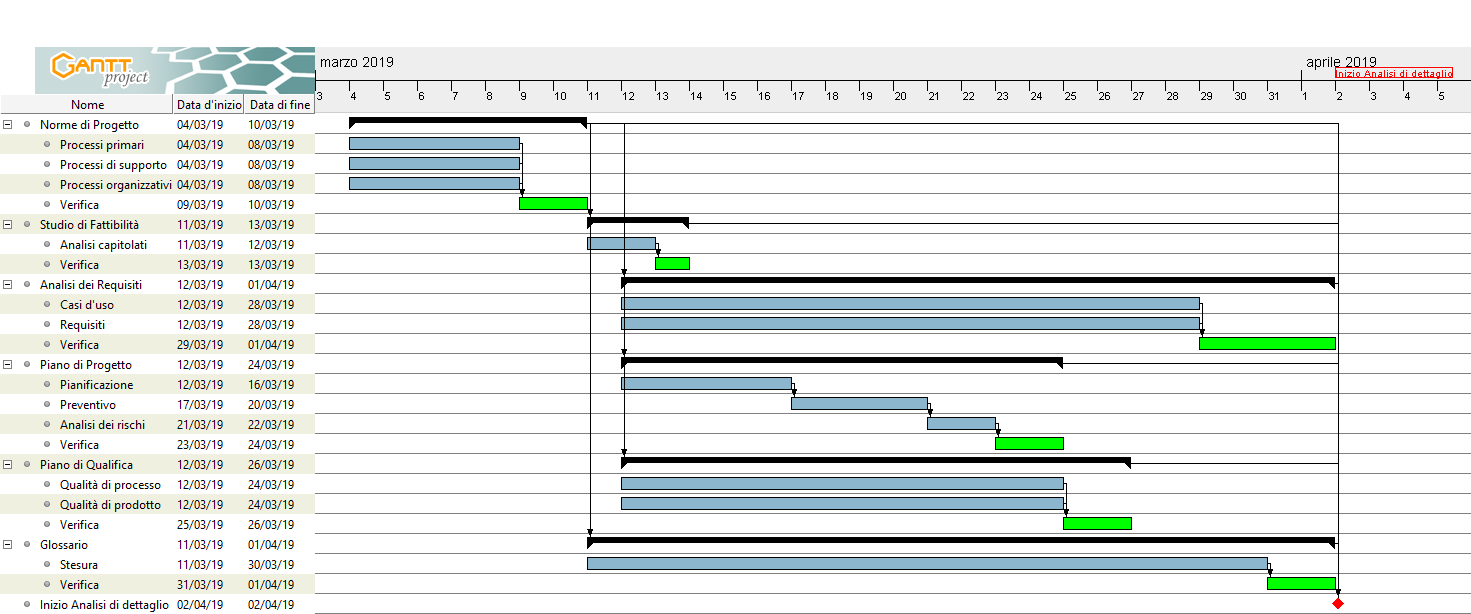
\includegraphics[scale=0.285]{immagini/AnalisiGantt.png}
  \caption{Diagramma di Gantt per la fase di Analisi}
  \end{center}
\end{figure}

\newpage

\subsection{Analisi di dettaglio}
La fase di Analisi di dettaglio ha inizio in data 02-04-2019 e termina il 19-04-2019, data in cui è stata fissata la prima Revisione dei Requisiti e in cui si svolgerà una presentazione del lavoro svolto nelle fasi di Analisi e, in parte, dell'Analisi di Dettaglio. In questo periodo le attività principali consistono nel miglioramento della qualità dei documenti tramite operazioni di incremento e verifica. Particolare attenzione è riservata all'attività di Analisi dei Requisiti che viene ulteriormente sviluppata consolidando i requisiti individuati da parte degli Analisti, successivamente ad incontri con il proponente del progetto. I ruoli attivi in questa fase sono:
\begin{itemize}
    \item \textbf{Responsabile di progetto};
    \item \textbf{Amministratore};
    \item \textbf{Verificatore};
    \item\textbf{Analista}.
\end{itemize}
Oltre all'incremento delle attività contenute nella fase di Analisi vengono aggiunte due nuove attività:
\begin{itemize}
    \item \textbf{Lettera di Presentazione}: Consiste nel redigere una lettera di presentazione, il cui scopo consiste nel presentare il team Cyber13 come fornitore del progetto scelto al proponente;
    \item \textbf{Presentazione}: Consiste nella preparazione dell'attività di presentazione per la Revisione dei Requisiti.
\end{itemize}
Tutte le attività, eccetto quella di Presentazione hanno termine massimo in data 12-04-2019, per cui è prevista la scadenza della consegna del materiale per accesso alla Revisione dei Requisiti.
\subsubsection{Diagramma di Gantt per la fase di Analisi di dettaglio}
\begin{figure}[h!]
\begin{center}
  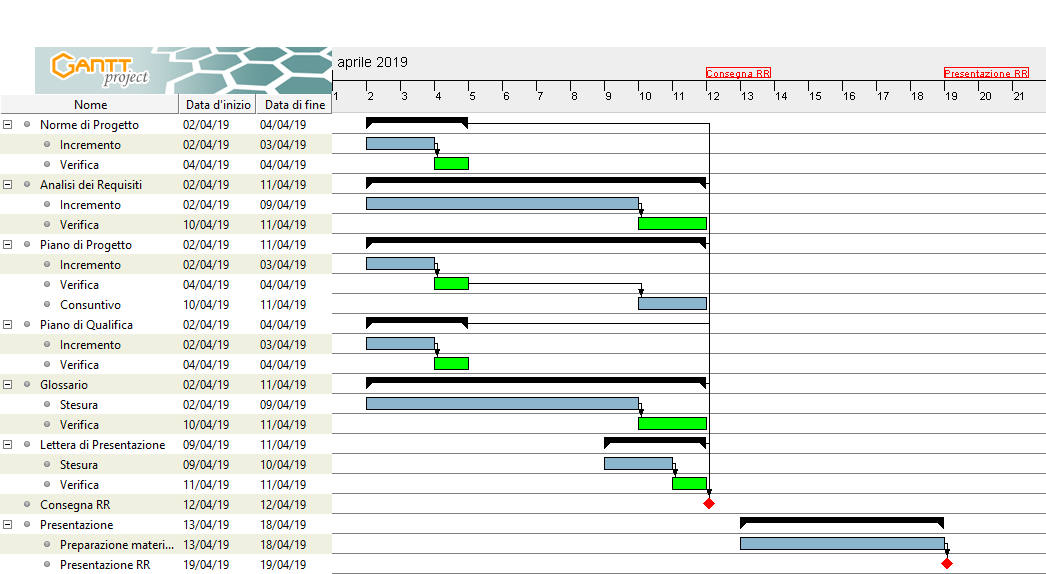
\includegraphics[scale=0.31]{immagini/AnalisiDettaglioGantt.png}
  \caption{Diagramma di Gantt per la fase di Analisi di dettaglio}
  \end{center}
\end{figure}

\newpage 

\subsection{Progettazione della base tecnologica}
La fase di Progettazione della base tecnologica ha inizio in data 20-04-2019 e termina il 17-05-2019. Ha inizio il giorno dopo la presentazione per la Revisione dei Requisiti e si conclude con la presentazione per la Revisione di Progettazione, previa consegna del materiale in data massima 10-05-2019.
I ruoli attivi in questa fase sono:
\begin{itemize}
    \item \textbf{Responsabile di progetto};
    \item \textbf{Amministratore};
    \item \textbf{Progettista};
    \item \textbf{Programmatore};
    \item \textbf{Verificatore};
    \item\textbf{Analista}.
\end{itemize}
Le attività svolte in questa fase sono le seguenti:
\begin{itemize}
    \item \textbf{Incremento e Verifica}: Vengono svolte attività di incremento e verifica sui documenti prodotti nelle fasi precedenti che necessitano di manutenzione per adattarli alle nuove attività (Norme di Progetto, Analisi dei Requisiti, Piano di Progetto, Piano di Qualifica);
    \item \textbf{Technology Baseline}: Consiste nella stesura del documento Technology Baseline da parte dei Progettisti. Tale documento conterrà le scelte progettuali ad alto livello effettuate dal team, oltre alla lista dei framework e delle librerie selezionate per lo sviluppo del prodotto. Questa attività risulta prioritaria durante questa fase dello sviluppo;
    \item \textbf{Proof of Concept}: Consiste nella realizzazione da parte dei programmatori di un piccolo prototipo basato sulle direttive del documento Technology Baseline a prova della validità delle scelte progettuali e tecnologiche effettuate;
    \item \textbf{Glossario}: Consiste nella manutenzione del documento Glossario, che per tutta la durata della fase sarà aggiornato tramite l'aggiunta di nuovi termini dove ritenuto necessario. Comprende anche il miglioramento dei contenuti già presenti;
    \item \textbf{Lettera di Presentazione}: Consiste nel redigere una lettera di presentazione allo scopo di presentare il gruppo per la Revisione di Progettazione;
    \item \textbf{Presentazione}: Consiste nella preparazione dell'attività di presentazione per la Revisione di Progettazione.
\end{itemize}
Tutte le attività, eccetto quella di Presentazione hanno termine massimo in data 10-05-2019, per cui è prevista la scadenza della consegna del materiale per accesso alla Revisione di Progettazione.
\subsubsection{Diagramma di Gantt per la fase di Progettazione della base tecnologica}
\begin{figure}[h!]
\begin{center}
  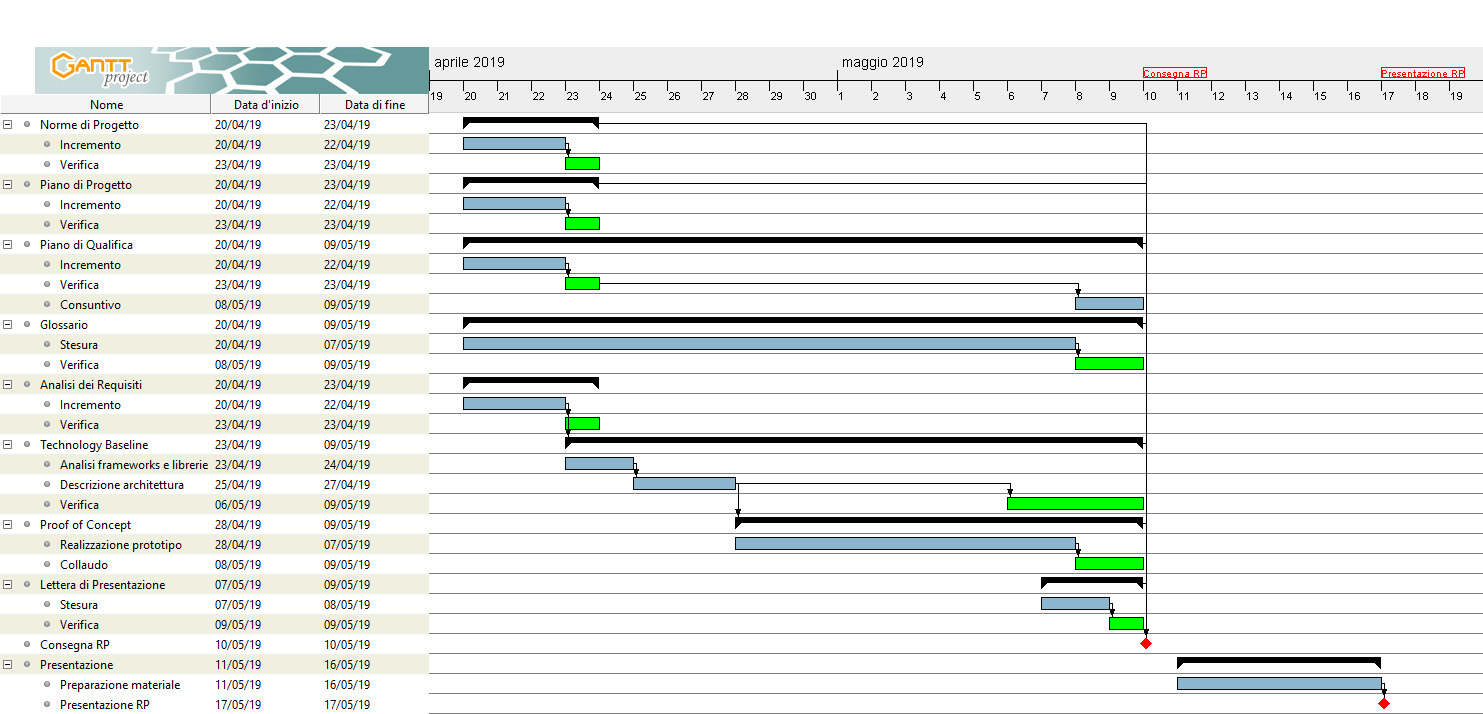
\includegraphics[scale=0.285]{immagini/ProgettazioneGantt.png}
  \caption{Diagramma di Gantt per la fase di Progettazione della base tecnologica}
  \end{center}
\end{figure}

\subsection{Progettazione di dettaglio e codifica}
La fase di Progettazione di dettaglio e codifica ha inizio in data 18-05-2019 e termina il 17-06-2019. Ha inizio il giorno dopo la presentazione per la Revisione di Progetto e si conclude con la presentazione per la Revisione di Qualifica, previa consegna del materiale in data massima 10-06-2019. 
I ruoli attivi in questa fase sono:
\begin{itemize}
    \item \textbf{Responsabile di progetto};
    \item \textbf{Amministratore};
    \item \textbf{Progettista};
    \item \textbf{Programmatore};
    \item \textbf{Verificatore};
    \item\textbf{Analista}.
\end{itemize}
Le attività svolte in questa fase sono le seguenti:
\begin{itemize}
    \item \textbf{Incremento e Verifica}: Vengono svolte attività di incremento e verifica sui documenti prodotti nelle fasi precedenti che necessitano di manutenzione per adattarli alle nuove attività (Norme di Progetto, Piano di Progetto, Piano di Qualifica e Technology Baseline);
    \item \textbf{Product Baseline}: Consiste nella stesura del documento Product Baseline da parte dei Progettisti. Tale documento contiene i dettagli della progettazione architetturale, tramite l'utilizzo di diagrammi delle classi e di sequenza, si deve basare sui contenuti del documento di Technology Baseline;
    \item \textbf{Codifica}: Consiste nella scrittura del codice dell'applicativo e nella sua successiva verifica. Deve basarsi su quanto riportato nel documento di Product Baseline. L'attività è svolta dagli Sviluppatori;
    \item \textbf{Manuale Utente}: Consiste nella stesura del documento Manuale Utente, contenente informazioni sull'utilizzo dell'applicativo prodotto dall'attività di Codifica;
    \item \textbf{Glossario}: Consiste nella manutenzione del documento Glossario, che per tutta la durata della fase sarà aggiornato tramite l'aggiunta di nuovi termini dove ritenuto necessario. Comprende anche il miglioramento dei contenuti già presenti;
    \item \textbf{Lettera di Presentazione}: Consiste nel redigere una lettera di presentazione allo scopo di presentare il gruppo per la Revisione di Qualifica;
    \item \textbf{Presentazione}: Consiste nella preparazione dell'attività di presentazione per la Revisione di Qualifica.
\end{itemize}
Tutte le attività, eccetto quella di Presentazione hanno termine massimo in data 10-06-2019, per cui è prevista la scadenza della consegna del materiale per accesso alla Revisione di Progettazione.
\subsubsection{Diagramma di Gantt per la fase di Progettazione di dettaglio e codifica}
\begin{figure}[h!]
\begin{center}
  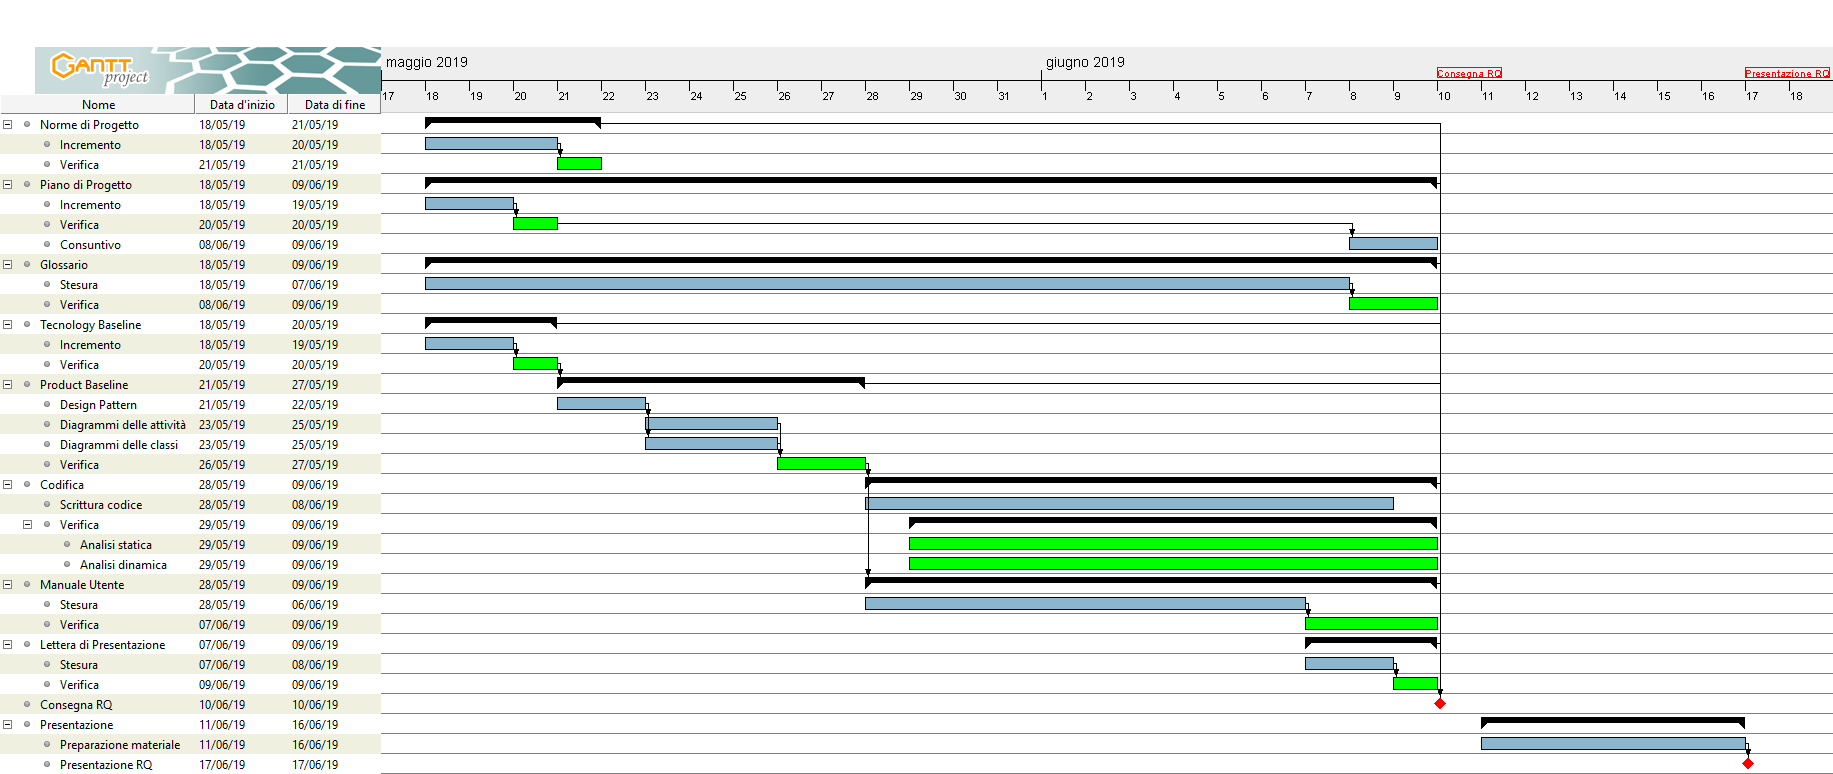
\includegraphics[scale=0.232]{immagini/CodificaGantt.png}
  \caption{Diagramma di Gantt per la fase di Progettazione di dettaglio e codifica}
  \end{center}
\end{figure}

\newpage

\subsection{Validazione e collaudo}
La fase di Progettazione di Validazione e collaudo ha inizio in data 18-06-2019 e termina il 15-07-2019. Ha inizio il giorno dopo la presentazione per la Revisione di Qualifica e si conclude con la presentazione per la Revisione di Accettazione, previa consegna del materiale in data massima 08-06-2019.
I ruoli attivi in questa fase sono:
\begin{itemize}
    \item \textbf{Responsabile di progetto};
    \item \textbf{Amministratore};
    \item \textbf{Progettista};
    \item \textbf{Programmatore};
    \item \textbf{Verificatore}.
\end{itemize}
Le attività svolte in questa fase sono le seguenti:
\begin{itemize}
    \item \textbf{Incremento e Verifica}: Vengono svolte attività di incremento e verifica sui documenti prodotti nelle fasi precedenti che necessitano di manutenzione per adattarli alle nuove attività (Norme di Progetto, Piano di Progetto, Piano di Qualifica, Product Baseline);
    \item \textbf{Validazione}: Consiste nella verifica del software dell'applicativo, effettuata da parte dei Verificatori e Programmatori, per verificare di aver soddisfatto i requisiti individuati nel documento Analisi dei Requisiti e il rispetto delle metriche di qualità presenti nel documento Piano di Qualifica. I programmatori provvedono all'adeguamento del software ai requisiti richiesti;
    \item \textbf{Collaudo}: Consiste nel controllo della correttezza delle funzionalità del prodotto, che viene eseguito e testato in ogni funzionalità richiesta dal proponente. Nell'attività sono coinvolti verificatori e programmatori, al fine di correggere le problematiche nel codice dell'applicativo, se rilevate durante il collaudo;
    \item \textbf{Manuale Utente}: Consiste nel miglioramento e completamento del documento Manuale Utente;
    \item \textbf{Glossario}: Consiste nella manutenzione del documento Glossario, che per tutta la durata della fase sarà aggiornato tramite l'aggiunta di nuovi termini dove ritenuto necessario. Comprende anche il miglioramento dei contenuti già presenti;
    \item \textbf{Lettera di Presentazione}: Consiste nel redigere una lettera di presentazione allo scopo di presentare il prodotto finale alla Revisione di Accettazione;
    \item \textbf{Consegna}: Al termine delle attività di Validazione e Collaudo viene consegnato il prodotto completo, con relativa documentazione, al committente;
    \item \textbf{Presentazione}: Consiste nella preparazione dell'attività di presentazione per la Revisione di Accettazione.
\end{itemize}
Tutte le attività, eccetto quella di Presentazione hanno termine massimo in data 08-07-2019, per cui è prevista la scadenza della consegna del materiale per accesso alla Revisione di Progettazione.
\subsubsection{Diagramma di Gantt per la fase di Validazione e collaudo}

\begin{figure}[h!]
\begin{center}
  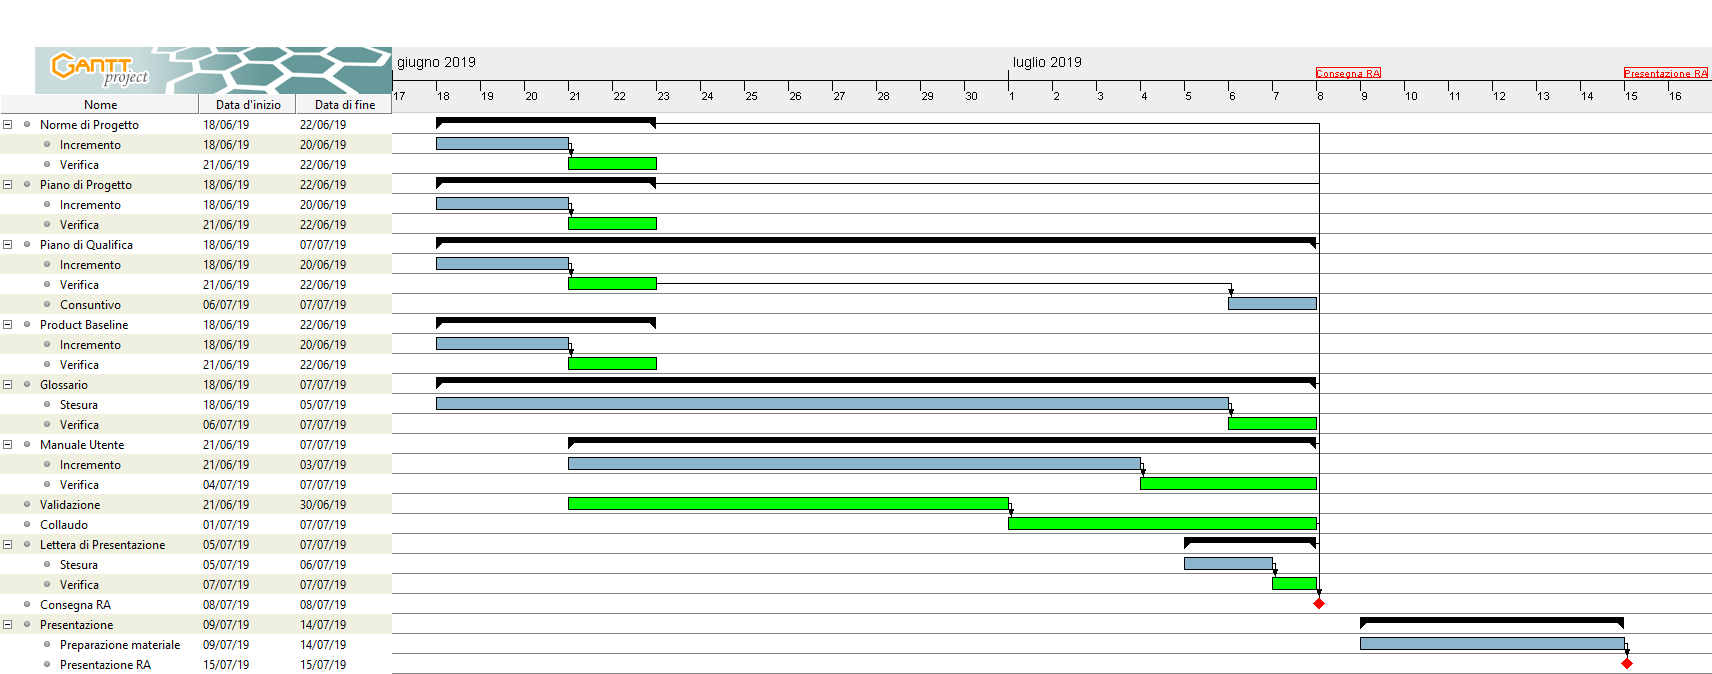
\includegraphics[scale=0.248]{immagini/ValidazioneGantt.png}
  \caption{Diagramma di Gantt per la fase di Validazione e collaudo}
  \end{center}
\end{figure}